% --------------------------------------------------------------------------
% Report template for BIR projects
% Report template with support for Portuguese and English languages
% Change language {brazil or english} in \documentclass as per the examples
% This template has support for the ABNT citing format
% 
% Original version: jan/2019
% https://github.com/
% 
% Based on ABNTEX2 and the thesis template
% --------------------------------------------------------------------------
\documentclass[
%\DeclareUnicodeCharacter{200B}{}
% --------------------------------------------------------------------------
% classe memoir . options                                                   
12pt,					% tamanho da fonte
openright,				% cap. começam em pág ímpar (ins pág vazia caso preciso)
twoside,				% para impressão em verso e anverso. Oposto a oneside
a4paper,				% tamanho do papel
% --------------------------------------------------------------------------
% classe abntex2 . options                                                  
%chapter=TITLE,			% títulos de capítulos convertidos em letras maiúsc.
%section=TITLE,			% títulos de seções convertidos em letras maiúsc.
%subsection=TITLE,		% títulos de subseções convertidos em letras maiúsc.
%subsubsection=TITLE,	% títulos de subsubseções convertidos em letras maiúsc.
% --------------------------------------------------------------------------
% Opções de IDIOMA do pacote babel                                          
english,
brazil
]{ABNT/abntex2_report}
% --------------------------------------------------------------------------
% Pacotes básicos    
\usepackage{lmodern}			% Usa a fonte Latin Modern			
\usepackage[T1]{fontenc}		% Selecao de codigos de fonte.
\usepackage[utf8]{inputenc}		% Codificacao do documento (conversão automática dos acentos)
\usepackage{indentfirst}		% Indenta o primeiro parágrafo de cada seção.
\usepackage{color}				% Controle das cores
\usepackage{graphicx}			% Inclusão de gráficos
\usepackage{microtype} 			% para melhorias de justificação
\usepackage{lipsum}	
\usepackage[brazilian,hyperpageref]{backref} % páginas com citações na bibliog.
%\usepackage[alf,abnt-etal-list=0,abnt-etal-cite=3,abnt-emphasize=bf]{abntex2cite}
\usepackage[alf]{abntex2cite}
%	
\usepackage{lastpage}			% Usado pela Ficha catalográfica
%\usepackage{subfig}
\usepackage{supertabular}       % tabela na capa do documento
\usepackage{booktabs}
\usepackage[table,xcdraw]{xcolor}
\usepackage{adjustbox}
\usepackage{amssymb,amsmath,mathrsfs}
\usepackage{algorithm,algpseudocode}
\usepackage{pgfplots}
\usepackage{tikz}
\usepackage{titlesec}
\usepackage{ragged2e}
\usepackage{tocloft}
\usepackage{threeparttable}
\usepackage{etoolbox}
\usepackage[normalem]{ulem}
\usepackage{yaacro}
\usepackage[none]{verlab}
%\usepackage{fontspec}
%\setmainfont{Helvetica Light}
\usepackage{lscape}
%\usepackage[graphicx]{realboxes}
\usepackage{rotating}
\usepackage{wrapfig}
\usepackage{caption}
\usepackage{subcaption}
\usepackage{dirtytalk}
\usepackage{pdfpages}
\usepackage{threeparttable}
\usepackage{hyperref}
%\hypersetup{draft}
\usepackage{float}
\DeclareUnicodeCharacter{200B}{}
% --------------------------------------------------------------------------%
% Configurações do PDF final                                                
\definecolor{blue}{RGB}{41,5,195}
\makeatletter
\hypersetup{
	%pagebackref=true,
	pdftitle={\@title}, 
	pdfauthor={\@author},
	pdfsubject={\@title},
	%pdfsubject={\imprimirpreambulo},
	pdfcreator={LaTeX with abnTeX2},
	pdfkeywords={abnt}{latex}{abntex}{abntex2}{\imprimirpalavraschave}, 
	colorlinks=true,       		% false: boxed links; true: colored links
	linkcolor=blue,          	% color of internal links
	citecolor=blue,        		% color of links to bibliography
	filecolor=magenta,      	% color of file links
	urlcolor=blue,
	bookmarksdepth=4
}
%\makeatother
% --------------------------------------------------------------------------
% Posiciona figuras e tabelas no topo da página quando adicionadas sozinhas
% em um página em branco. Ver https://github.com/abntex/abntex2/issues/170
%\makeatletter
\setlength{\@fptop}{5pt} % Set distance from top of page to first float
\makeatother
% --------------------------------------------------------------------------
% Formatação                                                                
\newcommand\tab[1][1cm]{\hspace*{#1}}
\apptocmd{\thebibliography}{\justifying}{}{} 
\renewcommand{\ABNTEXsectionfont}{\bfseries}
\titlespacing*{\chapter}{0pt}{0pt}{12pt}
\titlespacing*{\section}{0pt}{6pt}{6pt}
\titlespacing*{\subsection}{0pt}{6pt}{6pt}
\titlespacing*{\subsubsection}{0pt}{6pt}{6pt}
% --------------------------------------------------------------------------
% Rearranja os finais de cada estrutura                                     
\algrenewtext{EndWhile}{\algorithmicend\ \algorithmicwhile}
\algrenewtext{EndFor}{\algorithmicend\ \algorithmicfor}
\algrenewtext{EndIf}{\algorithmicend\ \algorithmicif}
\algrenewtext{EndFunction}{\algorithmicend\ \algorithmicfunction}
% --------------------------------------------------------------------------
% Espaçamentos entre linhas e parágrafos                                    
\setlength{\parindent}{1.3cm} % linha
\setlength{\parskip}{0.2cm} % parágrafo, tente também \onelineskip
% --------------------------------------------------------------------------
% Informações de dados para CAPA e FOLHA DE ROSTO                           
\prodtecnica{001 / 2020}
\titulo{Manipuladores inteligentes}
\tiporelatorio{Parcial} 
\nomeprojeto{Projeto}
\outrossubtitulos{~} % opcional
\autores{
	Moudu Zir\\
	Linki Terri\\
	Zakka Santi\\
	Toldu Jamou\\
	Maroc Sieru\
}
\newcommand{\autoresexternos}{
	John Marston\\
	Frank West\
}
\local{Salvador\\Bahia, Brasil}
\data{Abril de 2020}
\classificacao{( ) Confidencial  (X) Restrito  ( )  Uso Interno  ( ) Público}
\revisao{01}
\tabelacutter{000} 
\palavraschave{1. Manipulator. 2. Simulation. 3. Computer vision.}
\classificacaoassunto{000} % Número de Classificação do assunto 
%\parceirologo{logos/x.png}
%------------------------------------------------------------------
% Finalização das configurações da capa
%
%
%------------------------------------------------------------------              
% Acrônimos :: Chamar no texto como \ac{DoF}                                
\begin{acgroupdef}[list=acronyms]
	\acdef{DoF}{Degrees of Freedom}
	\acdef{PoC}{Proof of Concept, em português Prova de Conceito}
	\acdef{UUV}{Unmanned Underwater Vehicle, em português Veículo Subaquático Não-tripulado}
	\acdef{AUV}{Autonomous Underwater Vehicle, em português Veículo Subaquático Autônomo}
	\acdef{UVM}{Unmanned Vehicle Morphing}
	\acdef{SLAM}{Simultaneous Localization and Mapping}
	\acdef{ROV}{Remotely Operated Vehicle}
	\acdef{SOTA}{Study Of The Art}
	%
	%
	%
\end{acgroupdef}
% --------------------------------------------------------------------------
% Criação do sumário
\makeindex
%
\begin{document}
	\frenchspacing
	\imprimircapa
	\imprimircatalografica
% --------------------------------------------------------------------------
% Sumário executivo                                                         
	\ABNTEXchapterfont\large\textbf{\execsummarytitlename}
	\begin{flushleft}
		\normalsize
		\justify
		\normalfont
		O projeto de Manipuladores - Desafio.2, também conhecido como \textbf{xxxxx} se configura sob o Programa de Formação de Novos Talentos do Serviço Nacional de Aprendizagem Industrial, Departamento Regional da Bahia - Senai/DR/BA, sendo este o principal fomentador do programa.

		O projeto foi considerado como início técnico do projeto o dia 00 de bolsoneiro de 2020. 

		O prazo de execução planejado é de xx meses.
	\end{flushleft}
	\clearpage
%------------------------------------------------------------------
% Resumo e abstract                                                         
	\ABNTEXchapterfont\large\textbf{\resumoatitlename}
	\begin{flushleft}
		\normalsize
		\justify
		\normalfont
		%resumo aqui
		%
		%
		%
	\end{flushleft}
	\vspace*{1cm}
	\newpage
	%
	\ABNTEXchapterfont\large\textbf{\resumobtitlename}
	\begin{flushleft}
		\normalsize
		\justify
		\normalfont
		%abstract aqui
		%
		%
		%
	\end{flushleft}
	\clearpage
% --------------------------------------------------------------------------
% Lista de figuras                                                          
	\begin{flushleft}
		\ABNTEXchapterfont\Large\textbf{\MakeUppercase\listadefigurasname}
	\end{flushleft}
	\vspace*{-36pt}
	\pdfbookmark[0]{\listfigurename}{lof}
	\normalsize
	\listoffigures*
	\cleardoublepage
% --------------------------------------------------------------------------
% Lista de tabelas                                                          
	\begin{flushleft}
		\ABNTEXchapterfont\Large\textbf{\MakeUppercase\listadetabelasname}
	\end{flushleft}
	\vspace*{-36pt}
	\pdfbookmark[0]{\listtablename}{lot}
	\normalsize
	\listoftables*
	\cleardoublepage
% --------------------------------------------------------------------------
% Lista de símbolos e abreviaturas                                          
	\begin{flushleft}
	\ABNTEXchapterfont\Large\textbf{\MakeUppercase\listadesimbolsabrevtitlename}
		\noindent
		\vspace*{-06pt}
		\pdfbookmark[0]{\listadesiglasname}{lot}
		\normalsize
		\normalfont
		\aclist[list=acronyms]
	\end{flushleft}
	\newpage
% --------------------------------------------------------------------------
% Tabela de conteúdo                                                        	
	\begin{flushleft}
		\ABNTEXchapterfont\Large\textbf{\MakeUppercase\glosariotitlename}
	\end{flushleft}
	%\pagebreak
	\vspace*{-36pt}
	\pdfbookmark[0]{\contentsname}{toc}
	\normalsize
	\normalfont
	\tableofcontents*
	\justify
% --------------------------------------------------------------------------
% Formatação, remover espaço depois dos títulos
	\setlength\beforechapskip{-24pt}
	\setlength\afterchapskip{12pt}
	\textual
	\pagestyle{plain}
	\normalsize
	\justify
	\normalfont
% --------------------------------------------------------------------------
% Conteúdo do relatório  
	%SEÇÃO 1----------------------------------------------
\chapter{INTRODUÇÃO}
    Diferentes métodos constituem a prática da melhoria contínua. É de suma importância que os administradores conheçam estas ferramentas para que haja sempre redução de desperdícios, aumento da eficiência e controle dos processos.\cite{entenda_doe}

    Planejamento de Experimentos ou \ac{DOE}, é a técnica usada para estudar um produto ou processo, e assim, identificar os fatores que mais influenciam seu comportamento. Através deste método deve-se obter a mais otimizada configuração para a construção da peça ou elaboração do procedimento.\cite{oquee_doe}

    O desenvolvimento de um experimento bem executado deve explicitar os fatores-chave do processo, assim como a combinação dos fatores que fazem o processo funcionar de maneira aceitável. A variabilidade do processo, ou seja, a diferença entre o que esperamos de algo e o que realmente acontece também é um ponto a ser observado pelo executor do DOE.

    O resultado que determina uma característica ou elemento do experimento é chamado de \textbf{variável de resposta}. Por ser um método de abordagem repetitiva, é necessário realizar ciclos de testes para alcançar um bom resultado. Estes ciclos devem possuir três etapas: \textbf{Rastreamento} - fase de delimitação de variáveis e do campo de atuação; \textbf{Projeto fatorial completo} - fase de combinação de fatores e níveis de fatores e \textbf{Projeto de superfície}- Modelagem dos resultados obtidos.   

    O DOE pode ser aplicado em duas situações: planejamento de experimentos e correção de processos defeituosos. Um processo desenvolvido desde o início com esta aplicação garante que sua produção e gestão sejam sempre melhoradas e tenham custos e tempo reduzidos. É uma ferramenta de melhoria contínua bastante eficaz, desde que se tome os devidos cuidados com as etapas do experimento. \cite{oquee_doe}


    
    
    



	\chapter{CONCEITO DO SISTEMA}
\label{chap:conce}

%------------------------------------------------------------------
\section{Parâmetros básicos}
\label{sec:basi}


\subsection{Requisitos do cliente}
\label{sub:reqc}


\subsection{Requisitos técnicos}
\label{sub:reqt}


\subsection{Estudo do estado da arte}
\label{sub:sota}


\subsection{Ambiente de operação}
\label{sub:ambiente}


\subsection{Normas utilizadas}
\label{sub:normas}


\subsection{Benchmarking}
\label{sub:bench}


\subsection{Desdobramento da Função Qualidade}
\label{sub:qfd}


\subsection{Matriz morfológica}
\label{sub:matmorf}



	\chapter{DESENVOLVIMENTO DO SISTEMA}
\label{chap:desenv}


%------------------------------------------------------------------
\section{Descrição do sistema}
\label{sec:descsis}

\subsection{Arquitetura geral}
\label{sub:arqg}

\subsection{Especificação técnica}
\label{sub:esptec}

\subsection{Estrutura analítica do protótipo}
\label{sub:eap}



%------------------------------------------------------------------
\section{Especificação funcional} %na introdução da seção apresentar a conexão entre as funcionalidades
\label{sec:sota}



\subsection{Funcionalidade A}
\label{sub:funcA}
%aqui vc apresenta a funcionalidade

\subsubsection{Descrição} %incluir o fluxograma da funcionalidade aqui
\label{ssub:descA}

\subsubsection{Premissas necessárias}
\label{ssub:premA}

\subsubsection{Dependências}
\label{ssub:depA}

\subsubsection{Saídas}
\label{ssub:saidaA}



\subsection{Funcionalidade B}
\label{sub:funcB}

\subsubsection{Descrição} %incluir o fluxograma da funcionalidade aqui
\label{ssub:descB}

\subsubsection{Premissas necessárias}
\label{ssub:premB}

\subsubsection{Dependências}
\label{ssub:depB}

\subsubsection{Saídas}
\label{ssub:saidaB}


%------------------------------------------------------------------
\section{Arquitetura de software}
\label{sec:arqs}
%introdução ao assunto apresentando a arquitetura


\subsection{Diagrama de componentes}
\label{sub:diagcomp}


\subsection{Matriz de rastreabilidade de testes}
\label{sub:matrast}


%------------------------------------------------------------------
\section{Simulação do sistema}
\label{sec:simul}


\section{Integração}
\label{sec:integra}



\section{Testes realizados}
\label{sec:testes}









	\chapter{INTERPRETAÇÃO DOS RESULTADOS OBTIDOS}
\label{chap:resultados}
O modelo linear encontrado, considerando a interação entre dois elementos, é disposto a seguir.

\begin{knitrout}
\definecolor{shadecolor}{rgb}{0.969, 0.969, 0.969}\color{fgcolor}\begin{kframe}
\begin{verbatim}
## Call:
## lm(formula = score ~ (altura + clipe + ad_top + ad_left + ad_right) + 
##     altura * clipe + altura * ad_top + altura * ad_left + altura * 
##     ad_right + clipe * ad_top + clipe * ad_left + clipe * ad_right + 
##     ad_top * ad_left + ad_top * ad_right + ad_left * ad_right, 
##     data = helicoptero)
## 
## Residuals:
##       Min        1Q    Median        3Q       Max 
## -0.180625 -0.055313 -0.009375  0.059687  0.120625 
## 
## Coefficients:
##                    Estimate Std. Error t value Pr(>|t|)    
## (Intercept)         1.60813    0.07069  22.750 1.30e-13 ***
## altura-             0.18625    0.07903   2.357  0.03151 *  
## clipe-             -0.42375    0.07903  -5.362 6.36e-05 ***
## ad_top-             0.00375    0.07903   0.047  0.96274    
## ad_left-            0.14125    0.07903   1.787  0.09284 .  
## ad_right-           0.18625    0.07903   2.357  0.03151 *  
## altura-:clipe-     -0.03250    0.07069  -0.460  0.65186    
## altura-:ad_top-    -0.03750    0.07069  -0.531  0.60304    
## altura-:ad_left-    0.06750    0.07069   0.955  0.35382    
## altura-:ad_right-  -0.14250    0.07069  -2.016  0.06092 .  
## clipe-:ad_top-      0.09500    0.07069   1.344  0.19771    
## clipe-:ad_left-    -0.04000    0.07069  -0.566  0.57932    
## clipe-:ad_right-   -0.02000    0.07069  -0.283  0.78085    
## ad_top-:ad_left-   -0.13500    0.07069  -1.910  0.07425 .  
## ad_top-:ad_right-  -0.00500    0.07069  -0.071  0.94448    
## ad_left-:ad_right- -0.21000    0.07069  -2.971  0.00901 ** 
## ---
## Signif. codes:  0 '***' 0.001 '**' 0.01 '*' 0.05 '.' 0.1 ' ' 1
## 
## Residual standard error: 0.09996 on 16 degrees of freedom
## Multiple R-squared:  0.9161,	Adjusted R-squared:  0.8375 
## F-statistic: 11.65 on 15 and 16 DF,  p-value: 6.57e-06
\end{verbatim}
\end{kframe}
\end{knitrout}

Pode-se observar que para este modelo os elementos que possuem importância estatística, ou seja Pr $<$ 0.05 são: altura (Pr = 0.03151), clipe (Pr = 6.36e-05), ad\_right (Pr = 0.03151) e ad\_left:ad\_right (Pr = 0.00901). 

Considerando os elementos de importância estatística, a equação que representa o modelo é descrita da seguinte forma:

\begin{center}
$
  score = mean(scores) + \dfrac{coef(altura)}{2}altura + \dfrac{coef(clipe)}{2}clipe + \dfrac{coef(ad\_right)}{2}ad\_right +  \dfrac{ad\_left:ad\_right}{2}ad\_left:ad\_right
$  
\end{center}

Desta forma, fazendo as devidas substituições, temos que:

\begin{center}
  $
    score = 1.54 + \dfrac{0.18625}{2}altura + \dfrac{-0.42375}{2}clipe + \dfrac{0.18625}{2}ad\_right +  \dfrac{-0.21}{2}ad\_left:ad\_right
  $  

  $ score = 1.54 + 0.0931altura- 0.2119clipe + 0.0931ad\_right - 0.105ad\_left:ad\_right$

  $score\_max =  1.54 + 0.0931*(1)- 0.2119*(-1) + 0.0931*(1) - 0.105*(-1) = 2.04$

  $score\_min =  1.54 + 0.0931*(-1)- 0.2119*(1) + 0.0931*(-1) - 0.105*(1) = 1.04$
  \end{center}

	\chapter{CONFIABILIDADE DO SISTEMA}
\label{chap:conf}

%------------------------------------------------------------------
\section{Análise dos modos e efeitos de falhas}
\label{sec:fmeca}

%------------------------------------------------------------------
\section{Diagrama de blocos da Confiabilidade}
\label{sec:diag}

%------------------------------------------------------------------
\section{Análise da árvore de falhas}
\label{sec:fta}


	\chapter{GESTÃO DO CONHECIMENTO}
\label{chap:conhec}

%------------------------------------------------------------------
\section{Lições aprendidas}
\label{sec:licap}

%------------------------------------------------------------------
\section{Guia de uso}
\label{sec:guia}


	\chapter{CONCLUSÃO}
\label{chap:conclu}





	%\chapter{REFERENCIAL TEÓRICO}
\label{chap:refer}

%------------------------------------------------------------------
\section{Princípios de robótica}
\label{sec:princ}



	%\chapter{MATERIAIS E MÉTODOS}
\label{chap:metod}


%------------------------------------------------------------------
\section{Metodologia aplicada}
\label{sec:metaplic}




%------------------------------------------------------------------
\section{Especificação dos componentes utilizados} 
\label{sec:especif}



% --------------------------------------------------------------------------
% Referências
	\cleardoublepage
	\titleformat{\chapter}[display]{\vspace*{-24pt}\ABNTEXchapterfont\large\bfseries}{\chaptertitlename\ \thechapter}{12pt}{\Large}
	\bibliography{bibliography}
% --------------------------------------------------------------------------
% Apêndices
	\apendices
	\justify
	%
	\chapter{Questões de abordagem à pesquisa}
	\label{apend:quest}
	%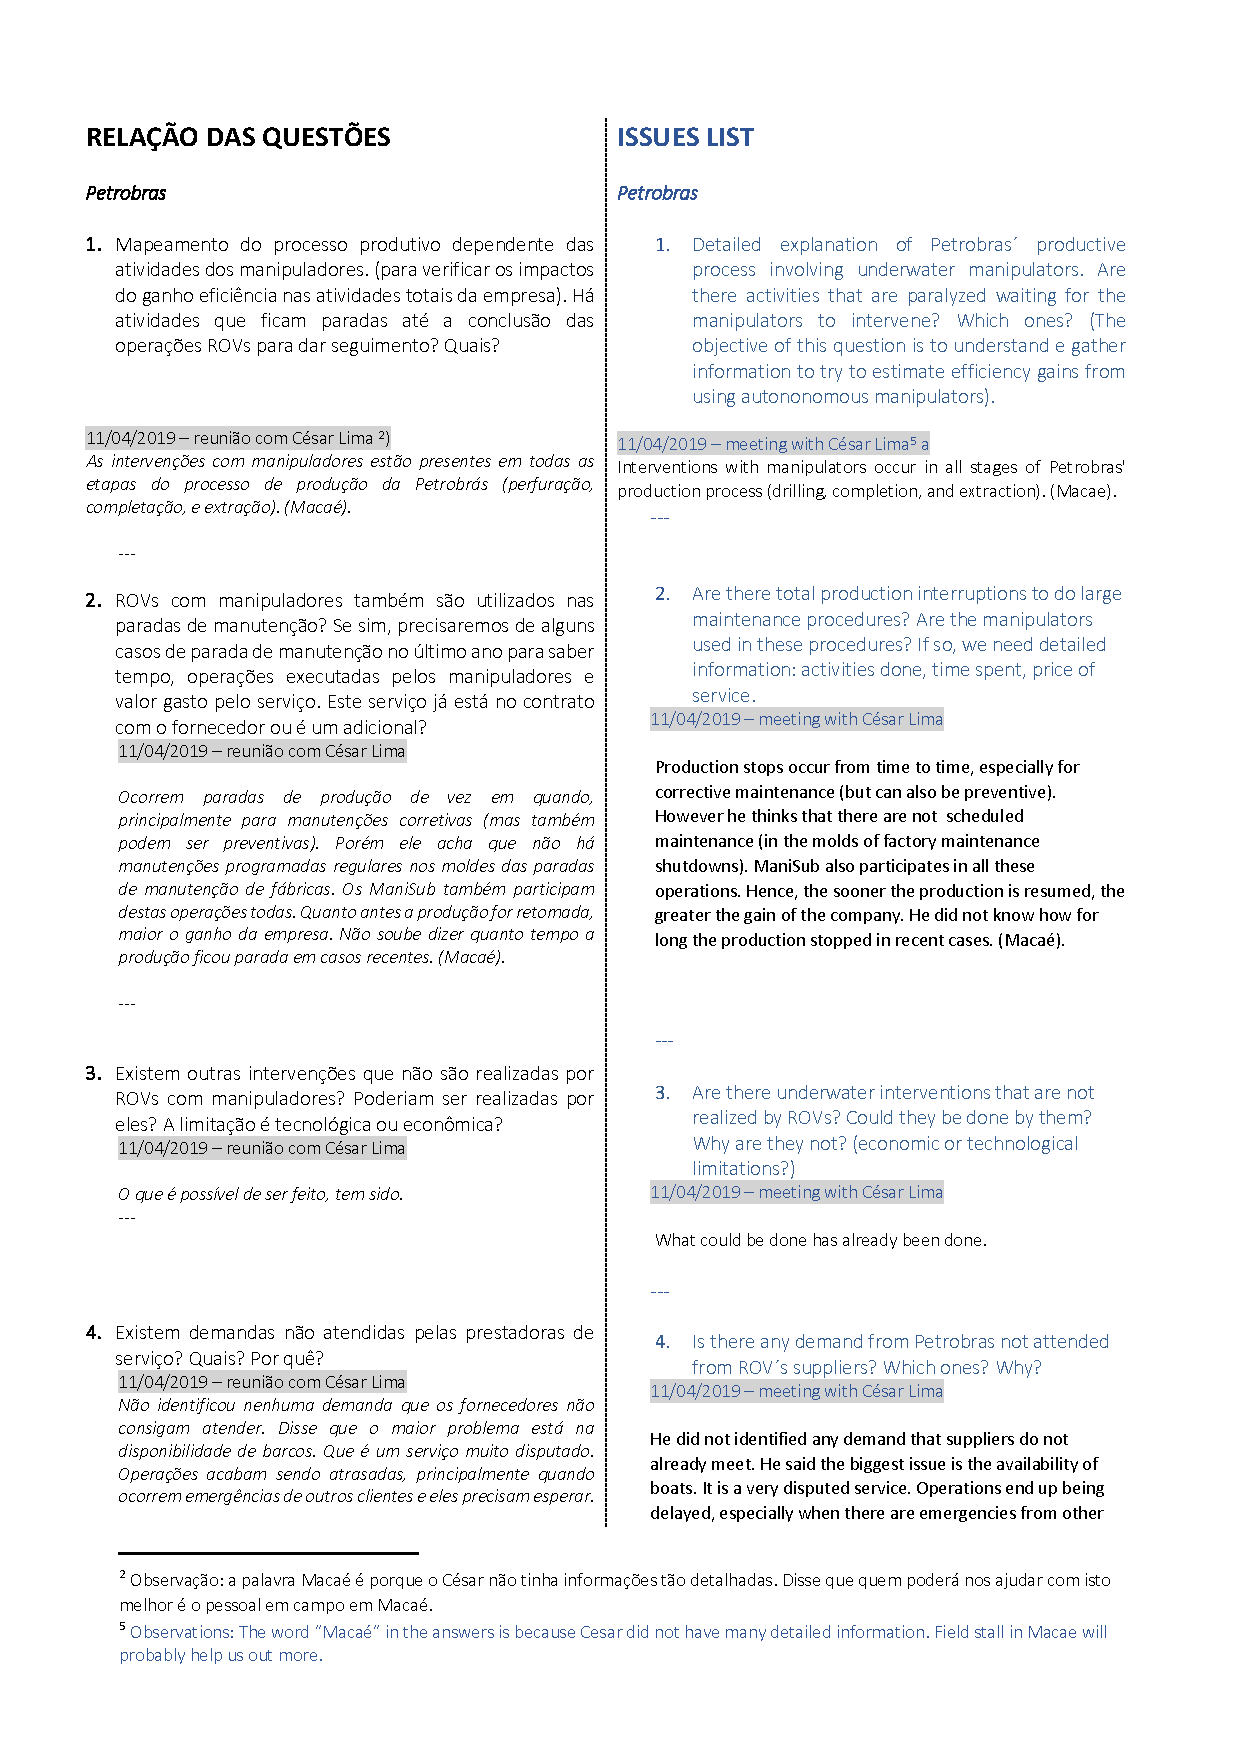
\includepdf[pages={{},-}]{appendix/listquest.pdf}
	\lipsum[1] % Comentar e adicionar apêndice aqui
	%
	\chapter{Um assunto importante}
	\label{apend:assunto}
	\lipsum[1] % Comentar e adicionar apêndice aqui
	

% --------------------------------------------------------------------------
% Anexos                                                                     
	\anexos
	\justify
	%
	\chapter{Outro assunto importante}
	\label{ann:relant}
	%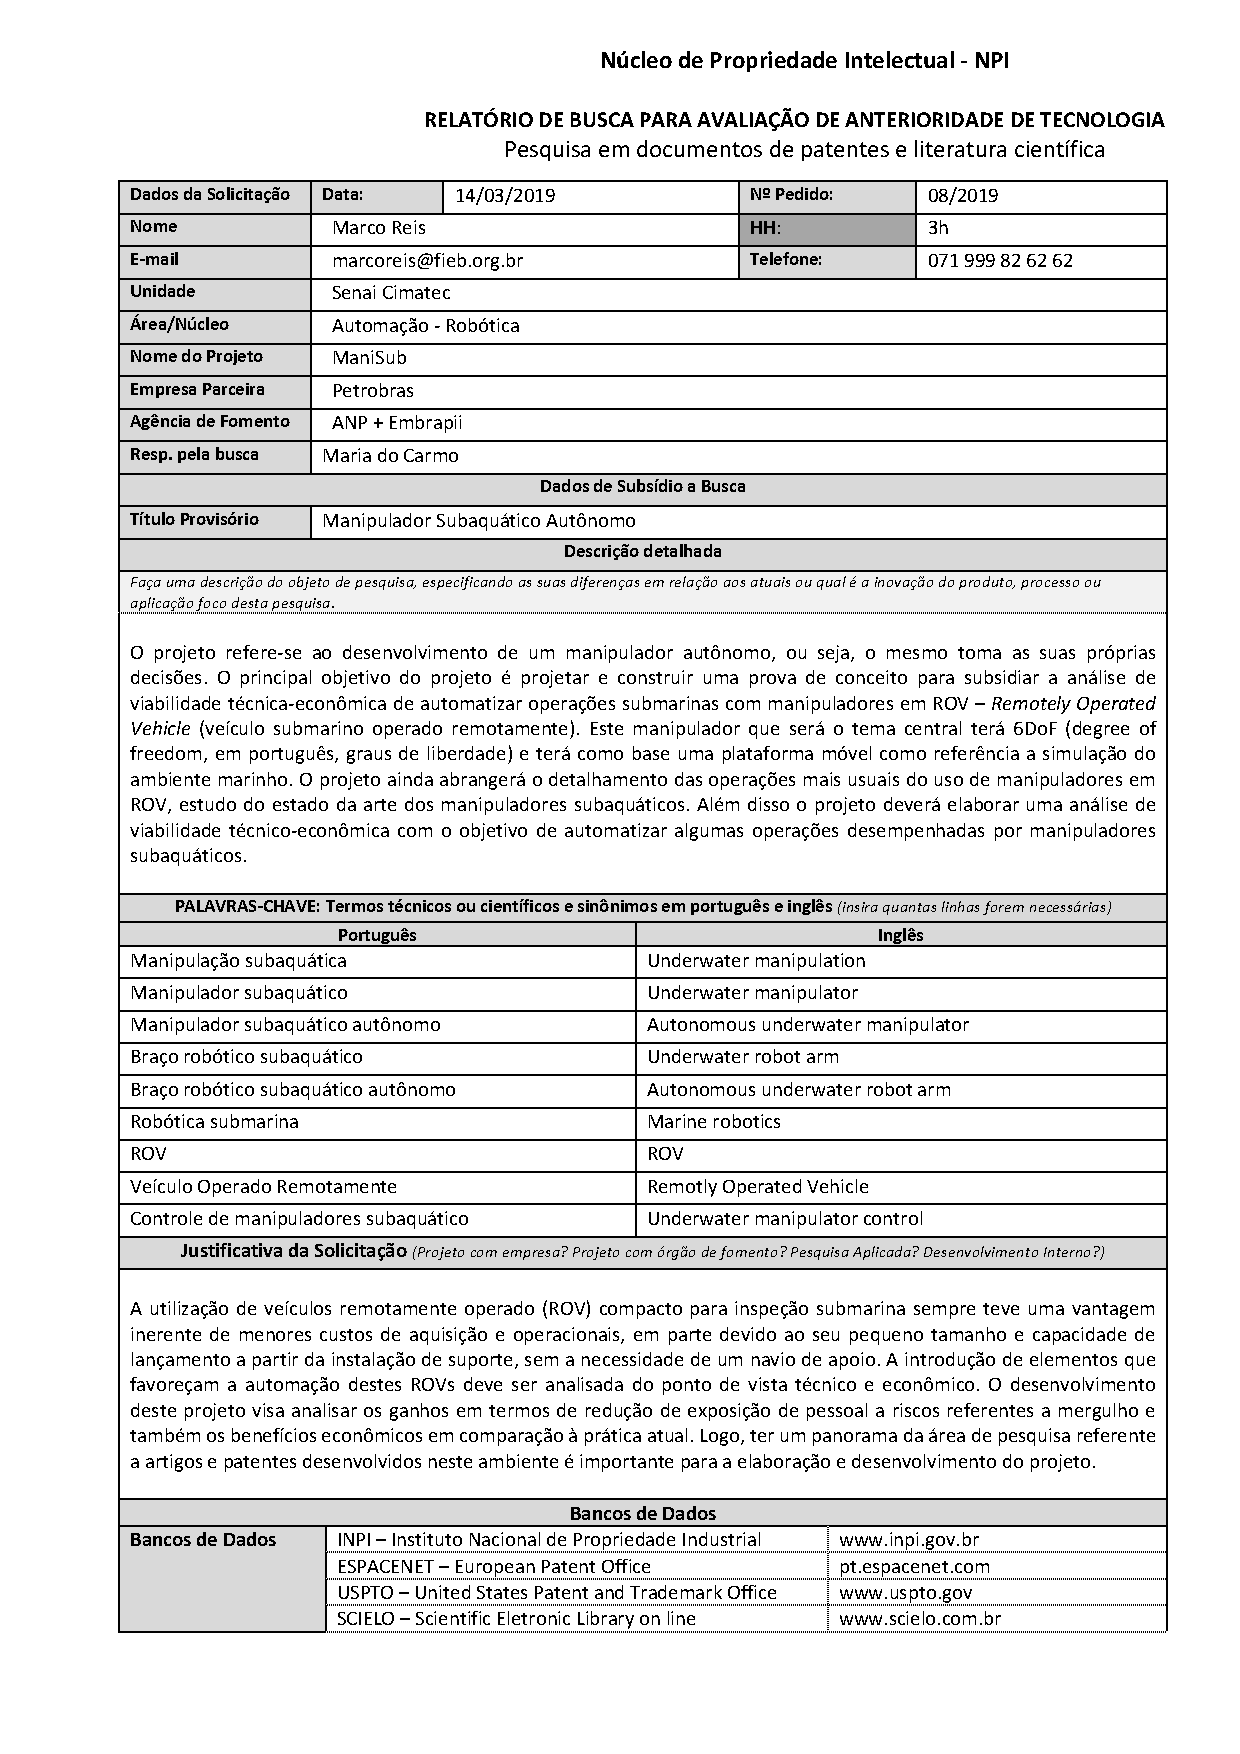
\includepdf[pages={{},-}]{annex/manisubanterioridade.pdf}
	\lipsum[1] % Comentar e adicionar apêndice aqui
	%
\end{document} 